\section{Time-Step Daylighting Calculation}\label{time-step-daylighting-calculation}

\subsection{Overview}\label{overview-027}

A daylighting calculation is performed each time step that the sun is up for each zone that has one or more daylighting reference points specified.
The exterior horizontal illuminance from the sun and sky is determined from solar irradiance data from the weather file.
The interior illuminance at each reference point is found for each window by interpolating the daylight illuminance factors for the current sun position, then,
for sky-related interior illuminance, multiplying by the exterior horizontal illuminance from the appropriate sky types that time step, and,
for sun-related interior illuminance, multiplying by the exterior horizontal solar illuminance that time step.
By summation, the net illuminance and glare due to all of the windows in a zone are found. 
If glare control has been specified window shading (by movable shading devices or switchable glazing) is deployed to reduce glare.
Finally the illuminance at each reference point for the final window and shade configuration is used by the lighting control system simulation
to determine the electric lighting power required to meet the illuminance setpoint at each reference point.

% table 27
\begin{longtable}[c]{p{1.0in}p{2.0in}p{1.0in}p{2.0in}}
\caption{Variables in Time-Step Calculations \label{table:variables-in-time-step-calculations}} \tabularnewline
\toprule 
Mathematical variable & Description & Units & C++ variable \tabularnewline
\midrule
\endfirsthead

\caption[]{Variables in Time-Step Calculations} \tabularnewline
\toprule 
Mathematical variable & Description & Units & C++ variable \tabularnewline
\midrule
\endhead

S\(_{norm,dir}\) & Direct normal solar irradiance & W/m\(^{2}\) & BeamSolarRad \tabularnewline
S\(_{h,dif}\) & Exterior diffuse horizontal solar irradiance & W/m\(^{2}\) & SDIFH, DifSolarRad \tabularnewline
S\(_{h,dir}\) & Exterior direct horizontal solar irradiance & W/m\(^{2}\) & SDIRH \tabularnewline
Z & Solar zenith angle & radians & Zeta \tabularnewline
m & Relative optical air mass & - & AirMass \tabularnewline
$\Delta$ & Sky brightness & - & SkyBrightness \tabularnewline
$\varepsilon$ & Sky clearness & - & SkyClearness \tabularnewline
k, k’ & Sky type index & - & ISky \tabularnewline
s\(_{k,k'}\) & Interpolation factor for skies k and k’ & - & SkyWeight \tabularnewline
$\psi$\(_{k,k'}\) & Sky luminance distribution formed from linear interpolation of skies k and k’ & cd/m\(^{2}\) & - \tabularnewline
f\(_{k}\) & Fraction of sky that is type k & - & - \tabularnewline
E\(_{h,k}\) & Horizontal illuminance from sky type k & cd/m\(^{2}\) & HorIllSky \tabularnewline
E\(_{h,sky}\) & Exterior horizontal illuminance from sky & lux & HISKF \tabularnewline
E\(_{h,sun}\) & Exterior horizontal illuminance from sun & lux & HISUNF \tabularnewline
$\eta$\(_{dif}\), $\eta$\(_{dir}\) & Luminous efficacy of diffuse and direct solar radiation & lm/W & DiffLumEff, DirLumEff \tabularnewline
I\(_{win}\) & Interior illuminance from a window & lux & DaylIllum \tabularnewline
S\(_{win}\) & Window luminance & cd/m\(^{2}\) & SourceLumFromWinAtRefPt \tabularnewline
B\(_{win}\) & Window background luminance & cd/m\(^{2}\) & BACLUM \tabularnewline
d\(_{sun}\), d\(_{sky,k}\) & Interior illuminance factor for sun, for sky of type k & - & DaylIllFacSun, DFSUHR, DaylIllFacSky, DFSUHR \tabularnewline
w\(_{sun}\), w\(_{sky,k}\) & Window luminance factor for sun, for sky of type k & - & DaylSourceFacSun, SFSUHR, DaylSourceFacSky, SFSKHR \tabularnewline
b\(_{sun}\), b\(_{sky,k}\) & Window background luminance factor for sun, for sky of type k & - & DaylBackFacSun, BFSUHR, DaylBackFacSky, BFSKHR \tabularnewline
w\(_{j}\) & Weighting factor for time step interpolation & - & WeightNow \tabularnewline
i\(_{L}\) & Reference point index & - & IL \tabularnewline
i\(_{S}\) & Window shade index & - & IS \tabularnewline
I\(_{tot}\) & Total daylight illuminance at reference point & lux & DaylIllum \tabularnewline
B\(_{tot}\), B & Total window background luminance & cd/m\(^{2}\) & BLUM \tabularnewline
I\(_{set}\) & Illuminance setpoint & lux & ZoneDaylight(ZoneNum).IllumSetPoint \tabularnewline
f\(_{L}\) & Fractional electric lighting output & - & FL \tabularnewline
f\(_{p}\) & Fractional electric lighting input power & - & FP \tabularnewline
N\(_{L}\) & Number of steps in a stepped control system & - & LightControlSteps \tabularnewline
M\(_{P}\) & Lighting power multiplier & - & ZonePowerReductionFactor \tabularnewline
\bottomrule
\end{longtable}

\subsection{Time-Step Sky Luminance}\label{time-step-sky-luminance}

The sky luminance distribution, \emph{$\psi$}, for a particular time step is expressed as a linear interpolation of two of the four standard skies --- \emph{$\psi$\(_{cs}\)}, \emph{$\psi$\(_{ts}\)} , \emph{$\psi$\(_{is}\)} and \emph{$\psi$\(_{os}\)} --- described above under ``Sky Luminance Distributions.'' The two sky types that are interpolated depend on the value of the sky clearness. The interpolation factors are a function of sky clearness and sky brightness (Perez et al., 1990). Sky clearness is given by:

\begin{equation}
\varepsilon  = \frac{{\frac{{{S_{h,dif}} + {S_{norm,dir}}}}{{{S_{h,dif}}}} + \kappa {Z^3}}}{{1 + \kappa {Z^3}}}
\end{equation}

where \emph{S\(_{h,dif}\)} is the diffuse horizontal solar irradiance, \emph{S\(_{norm,dir}\)} is the direct normal solar irradiance, \emph{Z} is the solar zenith angle and \emph{$\kappa$} is a constant equal to 1.041 for \emph{Z} in radians.

Sky brightness is given by:

\begin{equation}
\Delta  = {S_{h,dif}}m/S_{norm,dir}^{ext}
\end{equation}

where \emph{m} is the relative optical air mass and \(S_{norm,dir}^{ext}\) is the extraterrestrial direct normal solar irradiance.

The relative optional air mass is calculated as follows:

\begin{equation}
m = \frac{1- 1\mathrm{e}{-4}\cdot h}{\frac{\sin(b) + 0.15}{(b+3.885)^{1.253}}}
\end{equation}

where $b$ is the Solar Altitude Angle, that is the angle of the sun above the horizontal (in degrees), and $h$ is the building altitude (elevation, in meters).

\begin{equation}
b = \frac{\frac{\Pi}{2} - Z}{DegToRadians}
\end{equation}


If \emph{$\varepsilon$} $\leq$ 1.2,

\begin{equation}
{\psi_{is,os}} = {s_{is,os}}{\psi_{is}} + (1 - {s_{is,os}}){\psi_{os}}
\end{equation}

where \emph{$\psi$\(_{is}\)} is the intermediate sky luminance distribution, \emph{$\psi$\(_{os}\)} is the overcast sky luminance distribution, and

\begin{equation}
{s_{is,os}} = \min \{ 1,\max [0,(\varepsilon  - 1)/0.2,(\Delta  - 0.05)/0.4]\}
\end{equation}

If 1.2 \textless{}\emph{$\varepsilon$} $\leq$ 3

\begin{equation}
{\psi_{ts,is}} = {s_{ts,is}}{\psi_{ts}} + (1 - {s_{ts,is}}){\psi_{is}}
\end{equation}

where \emph{$\psi$\(_{ts}\)} is the clear turbid sky luminance distribution and

\begin{equation}
{s_{ts,is}} = (\varepsilon  - 1.2)/1.8
\end{equation}

If \emph{$\varepsilon$} \textgreater{} 3,

\begin{equation}
{\psi_{cs,ts}} = {s_{cs,ts}}{\psi_{cs}} + (1 - {s_{cs,ts}}){\psi_{ts}}
\end{equation}

where \emph{$\psi$\(_{cs}\)} is the clear sky luminance distribution and

\begin{equation}
{s_{cs,ts}} = \min [1,(\varepsilon  - 3)/3]
\end{equation}

\subsection{Interior Illuminance}\label{interior-illuminance}

For each time step the interior illuminance, \emph{I\(_{win}\)}, from a window is calculated as follows by multiplying daylight factors and exterior illuminance.

First, the sun- and sky-related daylight illuminance factors for the time step are determined by interpolation of the hourly factors:

\begin{equation}
{\bar d_{sun}}({i_L},{i_S}) = {w_j}{d_{sun}}({i_L},{i_S},{i_h}) + (1 - {w_j}){d_{sun}}({i_L},{i_S},{i_h} + 1)
\end{equation}

\begin{equation}
{\bar d_{sky,k}}({i_L},{i_S}) = {w_j}{d_{sky,k}}({i_L},{i_S},{i_h}) + (1 - {w_j}){d_{sky,k}}({i_L},{i_S},{i_h} + 1)
\end{equation}

where \emph{i\(_{L}\)} is the reference point index (1 or 2), \emph{i\(_{S}\)} is the window shade index (1 for unshaded window, 2 for shaded window), \emph{i\(_{h}\)} is the hour number, and \emph{k} is the sky type index. For the \emph{j\(^{th}\)} time step in an hour, the time-step interpolation weight is given by:

\begin{equation}
{w_j} = 1 - \min [1,j/{N_t}]
\end{equation}

where \emph{N\(_{t}\)} is the number of~ time steps per hour.

The interior illuminance from a window is calculated as:

\begin{equation}
{I_{win}}({i_L},{i_S}) = {\bar d_{sun}}{E_{h,sun}} + [{\bar d_{sky,k}}({i_L},{i_S}){f_k} + {\bar d_{sky,k'}}({i_L},{i_S}){f_{k'}}]{E_{h,sky}}
\end{equation}

where \emph{E\(_{h,sun}\)} and \emph{E\(_{h,sky}\)} are the exterior horizontal illuminance from the sun and sky, respectively, and \emph{f\(_{k}\)} and \emph{f\(_{k’}\)} are the fraction of the exterior horizontal illuminance from the sky that is due to sky type \emph{k} and \emph{k'}, respectively.

The horizontal illuminance from sun and sky are given by:

\begin{equation}
  \begin{array}{rl}
    E_{h,sun} & = \eta_{dir} S_{norm,dir} \cos Z \\
    E_{h,sky} & = \eta_{dif} S_{h,dif}
  \end{array}
\end{equation}

where \emph{Z} is the solar zenith angle,~ \emph{$\eta$\(_{dif}\)} is the luminous efficacy (in lumens/Watt) of diffuse solar radiation from the sky and \emph{$\eta$\(_{dir}\)} is the luminous efficacy of direct radiation from the sun. The efficacies are calculated from direct and global solar irradiance using a method described in (Perez et al, 1990), inside the DayltgLuminousEfficacy routine of the WeatherManager module.

The fractions \emph{f\(_{k}\)} and \emph{f\(_{k’}\)} are given by:

\begin{equation}
  \begin{array}{rl}
    f_k    & = \frac{ s_{k,k'} E_{h,k} } { s_{k,k'} E_{h,k} + (1 - s_{k,k'})E_{h,k'}} \\
    f_{k'} & = \frac{ (1 - s_{k,k'} ) E_{h,k'} } { s_{k,k'} E_{h,k} + (1 - s_{k,k'} ) E_{h,k'}}
  \end{array}
\end{equation}

where \emph{E\(_{h,k}\)} and \emph{E\(_{h,k’}\)} are the horizontal illuminances from skies \emph{k} and \emph{k'}, respectively (see ``Exterior Horizontal Luminance,'' above), and \emph{s\(_{k,k’}\)} is the interpolation factor for skies \emph{k}and \emph{k'}(see ``Time-Step Sky Luminance,'' above).~ For example, if~ \emph{$\varepsilon$} \textgreater{} 3, \emph{k} = \emph{cs} (clear sky), \emph{k'} = \emph{ts} (clear turbid sky) and

\begin{equation}
s_{k,k'} = s_{cs,ts} = \min [1,(\varepsilon - 3)/3]
\end{equation}

Similarly, the window source luminance, \emph{S\(_{win}\)}, and window background luminance, \emph{B\(_{win}\)}, for a window are calculated from

\begin{equation}
{S_{win}}({i_L},{i_S}) = {\bar w_{sun}}{E_{h,sun}} + [{\bar w_{sky,k}}({i_L},{i_S}){f_k} + {\bar w_{sky,k'}}({i_L},{i_S}){f_{k'}}]{E_{h,sky}}
\end{equation}

\begin{equation}
{B_{win}}({i_L},{i_S}) = {\bar b_{sun}}{E_{h,sun}} + [{\bar b_{sky,k}}({i_L},{i_S}){f_k} + {\bar b_{sky,k'}}({i_L},{i_S}){f_{k'}}]{E_{h,sky}}
\end{equation}

The total illuminance at a reference point from all of the exterior windows in a zone is

\begin{equation}
  {I_{tot}}({i_L}) = \sum\limits_{\genfrac{}{}{0pt}{2}{\rm{windows}}{\rm{in~zone}}} {{I_{win}}({i_s},{i_L})}
\end{equation}

where i\(_{S}\) = 1 if the window is unshaded and \emph{i\(_{S}\)} = 2 if the window is shaded that time step. (Before the illuminance calculation is done the window shading control will have been simulated to determine whether or not the window is shaded.)

Similarly, the total background luminance is calculated:

\begin{equation}
  {B_{tot}}({i_L}) = \sum\limits_{\genfrac{}{}{0pt}{2}{\rm{windows}}{\rm{in~zone}}} {{B_{win}}({i_s},{i_L})}
\end{equation}

\subsection{Glare Index}\label{glare-index-000}

The net glare index at each reference point is calculated as:

\begin{equation}
  {G_I}({i_L}) = 10{\log_{10}}\sum\limits_{\genfrac{}{}{0pt}{2}{\rm{windows}}{\rm{in~zone}}} {\frac{{{S_{win}}{{({i_L},{i_S})}^{1.6}}\Omega {{({i_L})}^{0.8}}}}{{B({i_L}) + 0.07\omega {{({i_L})}^{0.5}}{S_{win}}({i_L},{i_S})}}}
\end{equation}

where

\begin{equation}
B\left( {{i_L}} \right) = max\left( {{B_{win}}\left( {{i_L}} \right),{\rho_b}{I_{set}}\left( {{i_L}} \right)} \right)
\end{equation}

In the last relationship, the background luminance is approximated as the larger of the background luminance from daylight and the average background luminance that would be produced by the electric lighting at full power if the illuminance on the room surfaces were equal to the setpoint illuminance. In a more detailed calculation, where the luminance of each room surface is separately determined, \emph{B(i\(_{L}\))} would be better approximated as an area-weighted luminance of the surfaces surrounding a window, taking into account the luminance contribution from the electric lights.

\subsubsection{Glare Control Logic}\label{glare-control-logic}

If glare control has been specified and the glare index at either reference point exceeds a user-specified maximum value, \emph{G\(_{I,max}\)}, then the windows in the zone are shaded one by one in attempt to bring the glare at both points below \emph{G\(_{I,max}\)}. (Each time a window is shaded the glare and illuminance at each reference point is recalculated.) The following logic is used:

\begin{itemize}
\item
  If there is only one reference point, shade a window if it is unshaded and shading it decreases the glare, even if it does not decrease the glare below \emph{G\(_{I,max}\)}. Note that if a window~ has already been shaded, say to control solar gain, it will be left in the shaded state.

\item
  If there are two reference points, then:

  \begin{itemize}
  \tightlist
  \item
    If glare is too high at both points, shade the window if it decreases glare at both points.
  \item
    If glare is too high only at the first point, shade the window if the glare at the first point decreases, and the glare at the second point stays below \emph{G\(_{I,max}\)}.
  \item
    If glare is too high only at the second point, shade the window if the glare at the second point decreases, and the glare at the first point stays below \emph{G\(_{I,max}\)}.
  \end{itemize}

\item
  Shades are closed in the order specified by the fenestration objects listed in the WindowShadingControl object until glare at both points is below \emph{G\(_{I,max}\)}, or until there are no more windows left to shade.

\end{itemize}

\subsection{Lighting Control System Simulation}\label{lighting-control-system-simulation}

Once the final daylight illuminance value at each reference point has been determined, the electric lighting control is simulated. The fractional electric lighting output, \emph{f\(_{L}\)}, required to meet the setpoint at reference point \emph{i\(_{L}\)} is given by

\begin{equation}
{f_L}({i_L}) = {\rm{max}}\left[ {0,\frac{{{I_{set}}({i_L}) - {I_{tot}}({i_L})}}{{{I_{set}}({i_L})}}} \right]
\end{equation}

Here, \emph{I\(_{set}\)} is the illuminance setpoint and \emph{I\(_{tot}\)} is the daylight illuminance at the reference point. This relationship assumes that the electric lights at full power produce an illuminance equal to \emph{I\(_{set}\)} at the reference point.

The fractional electric lighting input power, \emph{f\(_{P}\)}, corresponding to \emph{f\(_{L}\)} is then calculated. The relationship between \emph{f\(_{P}\)} and \emph{f\(_{L}\)} depends on the lighting control type.

\subsubsection{Continuous Dimming Control}\label{continuous-dimming-control}

For a continuously-dimmable control system, it is assumed that \emph{f\(_{P}\)} is constant and equal to \emph{f\(_{P,min}\)}for \emph{f\(_{L}\)\textless{}f\(_{L,min}\)} and that f\(_{P}\) increases linearly from \emph{f\(_{P,min}\)} to 1.0 as \emph{f\(_{L}\)} increases from \emph{f\(_{L,min}\)} to 1.0 (Figure~\ref{fig:control-action-for-a-continuous-dimming}). This gives:

\begin{equation}
  f_P = \left\{
          \begin{array}{cl}
            f_{P,min} & for~f_L < f_{L,min} \\
            \frac{f_L + (1 - f_L)f_{P,min} - f_{L,min}}{1 - f_{L,min}} & for~f_{L,min} \le f_L \le 1
          \end{array}
        \right.
\end{equation}

\begin{figure}[hbtp] % fig 60
\centering
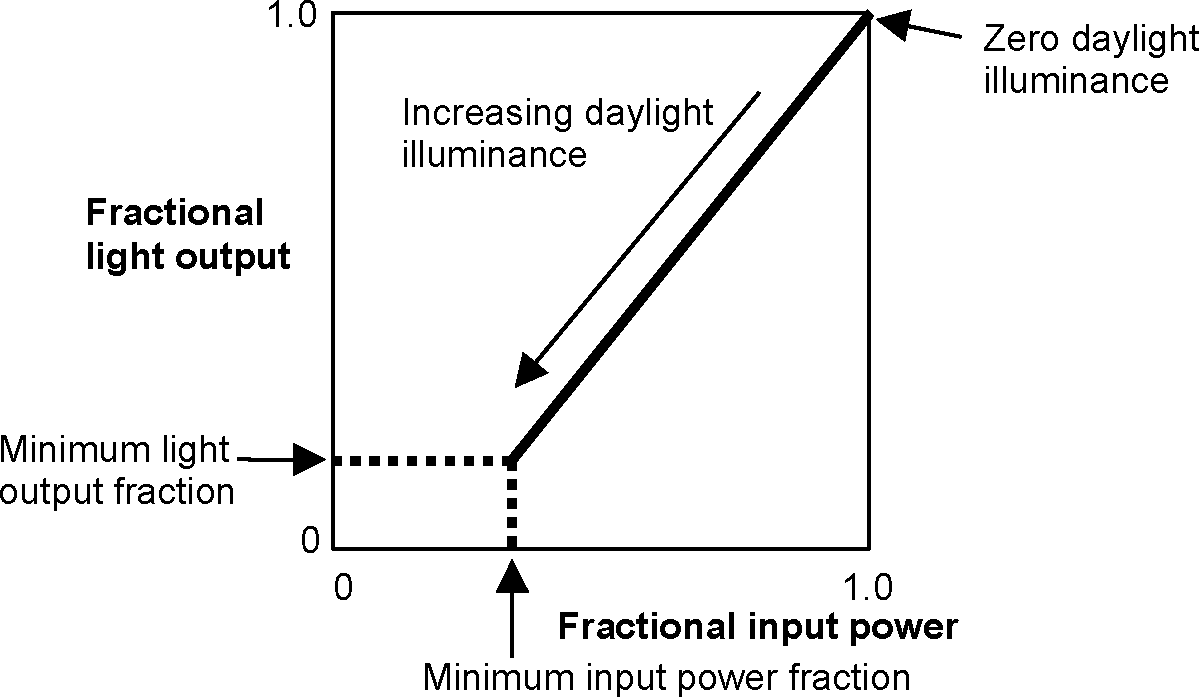
\includegraphics[width=0.9\textwidth, height=0.9\textheight, keepaspectratio=true]{media/image823.png}
\caption{Control action for a continuous dimming system. \protect \label{fig:control-action-for-a-continuous-dimming}}
\end{figure}

\subsubsection{Continuous/Off Dimming Control}\label{continuousoff-dimming-control}

A ``continuous/off'' dimming system has the same behavior as a continuous dimming system except that the lights switch off for \emph{f\(_{L}\) \textless{} f\(_{L,min}\)} rather than staying at \emph{f\(_{P,min}\)}.

\subsubsection{Stepped Control}\label{stepped-control}

For a stepped control system, \emph{f\(_{P}\)} takes on discrete values depending on the range of \emph{f\(_{L}\)} and the number of steps, \emph{N\(_{L}\)} (Figure~\ref{fig:stepped-lighting-control-with-three-steps.}). This gives:

\begin{equation}
  f_P = \left\{
          \begin{array}{cl}
            0 & for~f_L = 0 \\
            \frac{\mathop{\rm int} (N_L f_L) + 1}{N_L} & for~0 < f_L < 1 \\
            1 & for~f_L = 1
          \end{array}
         \right.
\end{equation}

If a lighting control probability, $P_L$, is specified, $f(P)$ is set one level higher a fraction of the time equal to $1-p(L)$. Specifically, if $f_P<1$, $f_P = f_P+1/N_L$ if a random number between 0 and 1 exceeds $p_L$. This can be used to simulate the uncertainty associated with manual switching of lights.

\begin{figure}[hbtp] % fig 61
\centering
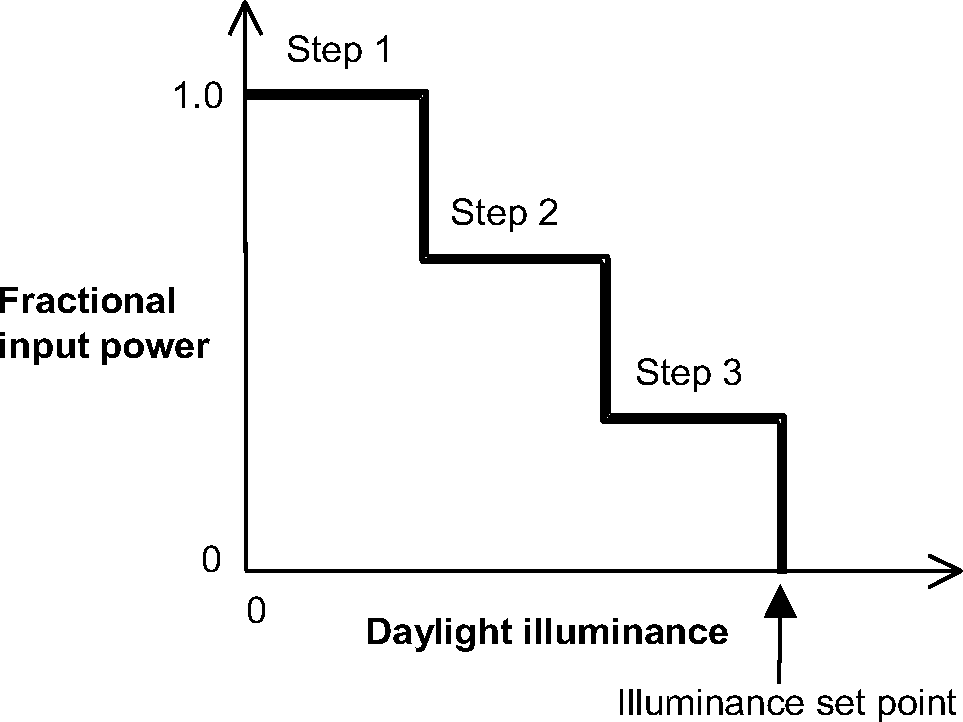
\includegraphics[width=0.9\textwidth, height=0.9\textheight, keepaspectratio=true]{media/image825.png}
\caption{Stepped lighting control with three steps. \protect \label{fig:stepped-lighting-control-with-three-steps.}}
\end{figure}

\subsubsection{Lighting Power Reduction}\label{lighting-power-reduction}

Using the value of \emph{f\(_{P}\)} at each reference point and the fraction \emph{f\(_{Z}\)} of the zone controlled by the reference point, the net lighting power multiplier, \emph{M\(_{P}\)}, for the entire zone is calculated; this value multiplies the lighting power output without daylighting.

\begin{equation}
{M_P} = \sum\limits_{{i_L} = 1}^2 {{f_P}({i_L})} {f_Z}({i_L}) + \left( {1 - \sum\limits_{{i_L} = 1}^2 {} {f_Z}({i_L})} \right)
\end{equation}

In this expression, the term to the right in the parentheses corresponds to the fraction of the zone not controlled by either reference point. For this fraction the electric lighting is unaffected and the power multiplier is 1.0.

\subsection{References}\label{references-045}

CIE Technical Committee 4.2. 1973. Standardization of the Luminance Distribution on Clear Skies. CIE Pub. No. 22, Commission Internationale d'Eclairage, Paris.

Hopkinson, R.G., J. Longmore and P. Petherbridge. 1954. An Empirical Formula for the Computation of the Indirect Component of Daylight Factors. Trans. Illum. Eng. Soc. (London) 19, 201.

Hopkinson, R.G., P. Petherbridge and J. Longmore. 1966. Daylighting. Heinnemann, London, p.~322.

Hopkinson, R.G. 1970. Glare from Windows. Construction Research and Development Journal 2, 98.

Hopkinson, R.G. 1972. Glare from Daylighting in Buildings. Applied Ergonomics 3, 206.

Kittler, R. 1965. Standardization of Outdoor Conditions for the Calculation of the Daylight Factor with Clear Skies. Proc. CIE Inter-Session Meeting on Sunlight, Newcastle-Upon-Tyne.

Lynes, J.A. 1968. Principles of Natural Lighting. Applied Science Publishers, Ltd., London, p.~129.

Matsuura, K. 1987. Luminance Distributions of Various Reference Skies. CIE Technical Report of TC 3-09.

Moon, P. and D. Spencer. 1942. Illumination from a Nonuniform Sky. Illuminating Engineering 37, 707-726.

Perez, R., P. Ineichen, R. Seals, J. Michalsky and R. Stewart. 1990. Modeling Daylight Availability and Irradiance Components from Direct and Global Irradiance. Solar Energy 44, 271-289.

Petherbridge, P. and J. Longmore. 1954. Solid Angles Applied to Visual Comfort Problems. Light and Lighting 47,173.

Winkelmann, F.C.~ 1983. Daylighting Calculation in DOE-2\emph{.} Lawrence Berkeley Laboratory report no. LBL-11353, January 1983.

Winkelmann, F.C. and S. Selkowitz. 1985. Daylighting Simulation in the DOE-2 Building Energy Analysis Program\emph{.} Energy and Buildings 8, 271-286.
